\documentclass[a4paper,twoside,11pt]{article}
\usepackage{a4wide,graphicx,fancyhdr,amsmath,amssymb,placeins}
\usepackage{listings}
\usepackage{color}
\usepackage{enumitem}
\usepackage{amsmath}
\usepackage{textcomp}
\usepackage{caption,subcaption}

%----------------------- Macros and Definitions --------------------------

\setlength\headheight{20pt}
\addtolength\topmargin{-10pt}
\addtolength\footskip{20pt}

\newcommand{\N}{\mathbb{N}}
\newcommand{\ch}{\mathcal{CH}}
\newcommand{\cpp}{{\tt C++} }

\newcommand{\solution}[1]{\noindent{\bf Solution to Exercise #1:}}

\renewcommand{\lstlistingname}{Codeblock}
\captionsetup[lstlisting]{font={small,tt}}

\fancypagestyle{plain}{%
\fancyhf{}
\fancyhead[LO,RE]{\sffamily\bfseries\large technische universiteit eindhoven}
\fancyhead[RO,LE]{\sffamily\bfseries\large 2IW02 RTSD}
\fancyfoot[LO,RE]{\sffamily\bfseries\large department of mathematics and computer science}
\fancyfoot[RO,LE]{\sffamily\bfseries\thepage}
\renewcommand{\headrulewidth}{0pt}
\renewcommand{\footrulewidth}{0pt}
}

\pagestyle{fancy}
\fancyhf{}
\fancyhead[RO,LE]{\sffamily\bfseries\large technische universiteit eindhoven}
\fancyhead[LO,RE]{\sffamily\bfseries\large 2IW02 RTSD}
\fancyfoot[LO,RE]{\sffamily\bfseries\large department of mathematics and computer science}
\fancyfoot[RO,LE]{\sffamily\bfseries\thepage}
\renewcommand{\headrulewidth}{1pt}
\renewcommand{\footrulewidth}{0pt}

%-------------------------------- Title ----------------------------------

\title{\vspace{-\baselineskip}\sffamily\bfseries Exercise 1}
\author{
	Rick Veens \qquad Studentno: 0912292\\
	\texttt{r.veens@student.tue.nl}
	\and
	Huib Donkers \qquad Studentno: 0769015\\
	\texttt{h.t.donkers@student.tue.nl}
}

\date{\today}

\definecolor{listinggray}{gray}{0.9}
\definecolor{lbcolor}{rgb}{0.9,0.9,0.9}
\lstset{
backgroundcolor=\color{lbcolor},
    tabsize=4,    
%   rulecolor=,
    language=[GNU]C++,
        basicstyle=\scriptsize,
        upquote=true,
        aboveskip={1.5\baselineskip},
        columns=fixed,
        showstringspaces=false,
        extendedchars=false,
        breaklines=true,
        prebreak = \raisebox{0ex}[0ex][0ex]{\ensuremath{\hookleftarrow}},
        frame=single,
        numbers=left,
        showtabs=false,
        showspaces=false,
        showstringspaces=false,
        identifierstyle=\ttfamily,
        keywordstyle=\color[rgb]{0,0,1},
        commentstyle=\color[rgb]{0.026,0.112,0.095},
        stringstyle=\color[rgb]{0.627,0.126,0.941},
        numberstyle=\color[rgb]{0.205, 0.142, 0.73},
%        \lstdefinestyle{C++}{language=C++,style=numbers}’.
}

% geen stomme indents bij \par
\setlength{\parindent}{0cm}

%--------------------------------- Text ----------------------------------

\begin{document}
\maketitle

\section{}
\subsection{}
\subsubsection{}
We modelled the deadlock free system as show in figure~\ref{fig:SystemDF}, and the deadlocked system as shown in figure~\ref{fig:SystemDC}. As expected, FDR accepts the deadlock free system (firgure~\ref{fig:FDR_DF}), but not the deadlocked system (figure~\ref{fig:FDR_DC}).
\begin{figure}
 \centering
 \begin{subfigure}{\textwidth}
  \centering
  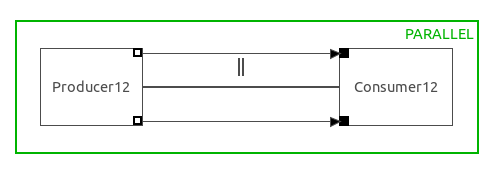
\includegraphics[scale=0.8]{./images/1_1-SystemDF_main.png}
  \caption{Composition of the Producer and Consumer processes.}
 \end{subfigure}
 \begin{subfigure}{0.5\textwidth}
  \centering
	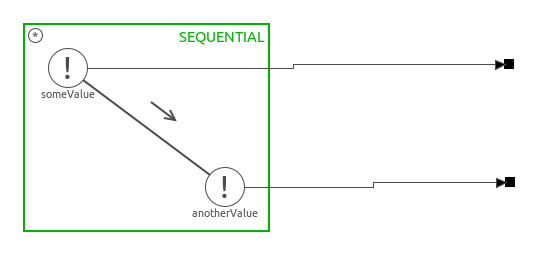
\includegraphics[scale=0.8]{./images/1_1-SystemDF_prod.png}
	\caption{The producer process.}
 \end{subfigure}%
 \begin{subfigure}{0.5\textwidth}
  \centering
	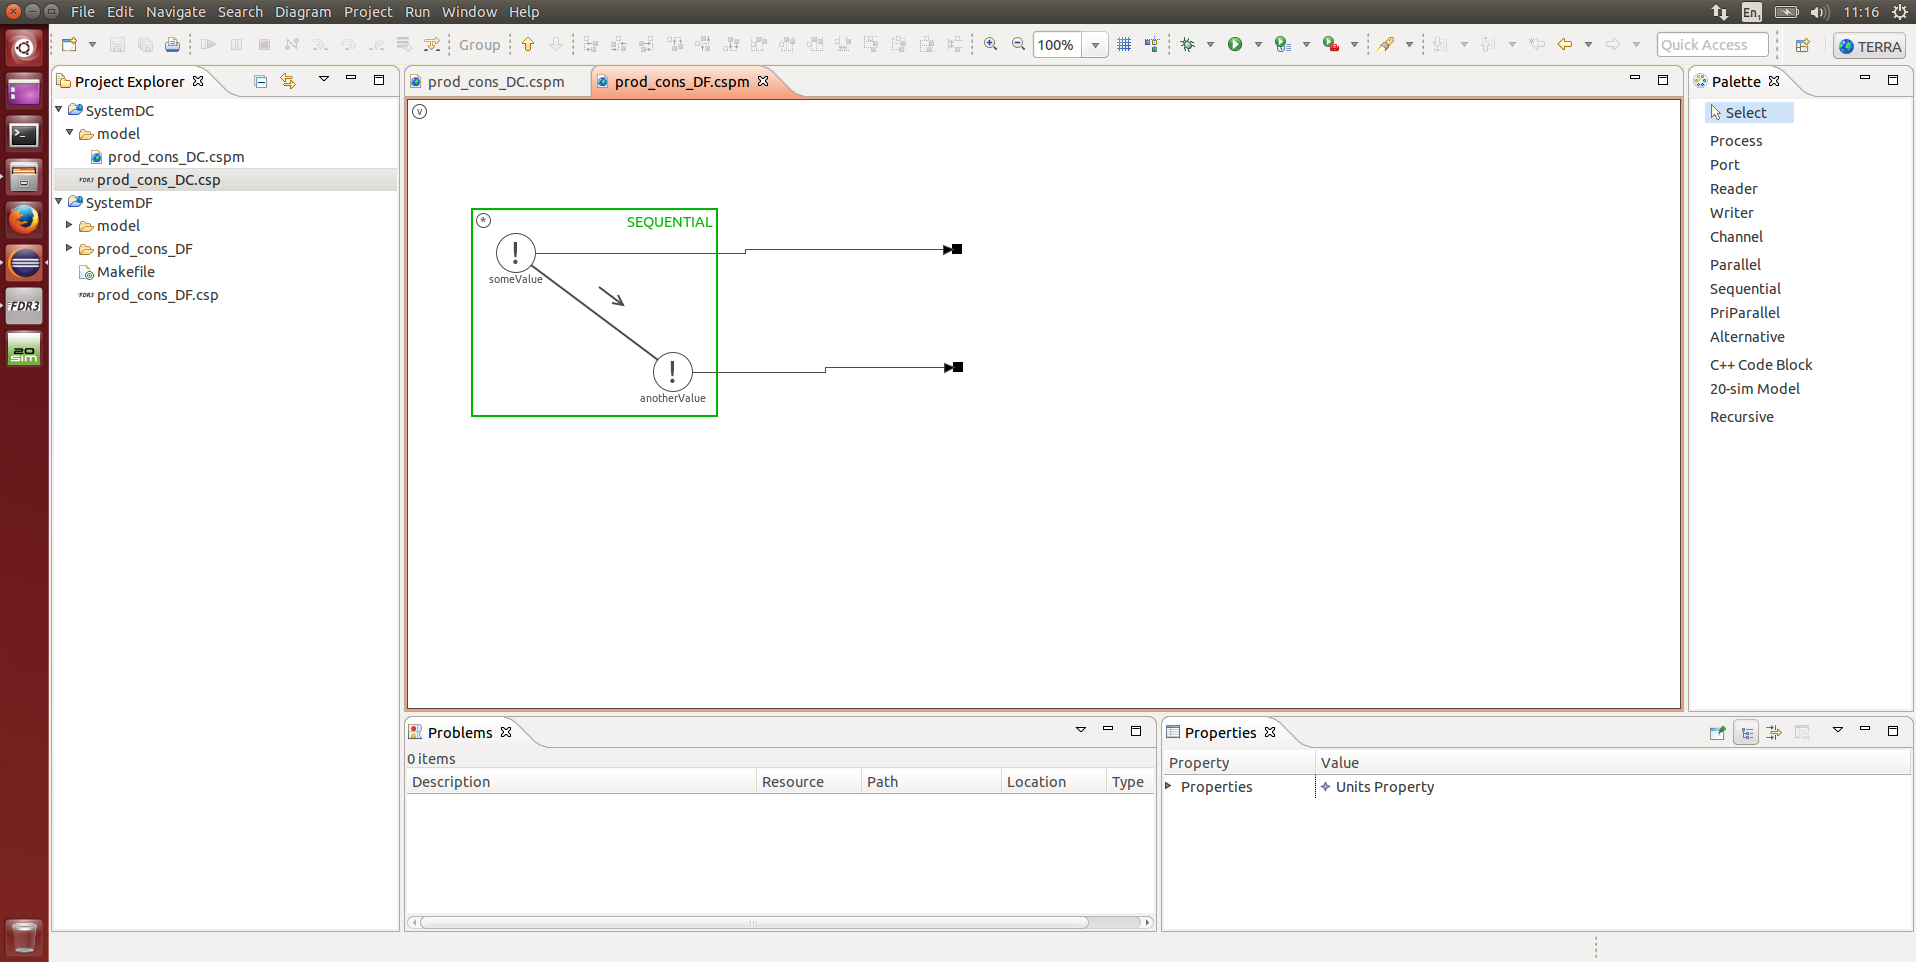
\includegraphics[scale=0.8]{./images/1_1-SystemDF_cons.png}
	\caption{The consumer process.}
 \end{subfigure}
 \caption{The producer-consumer (DF) model.}
 \label{fig:SystemDF}
\end{figure}

\begin{figure}
 \centering
 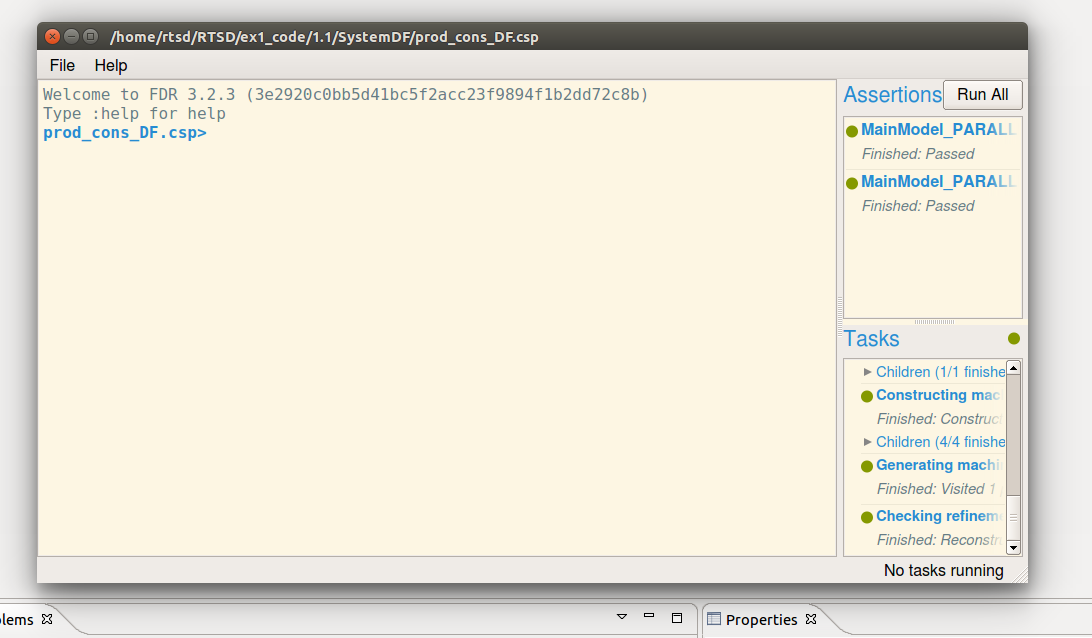
\includegraphics[width=\textwidth]{./images/1_1-SystemDF.png}
 \caption{Succesfully passes tests in FDR.}
 \label{fig:FDR_DF}
\end{figure}


\begin{figure}
 \centering
 \begin{subfigure}{\textwidth}
  \centering
  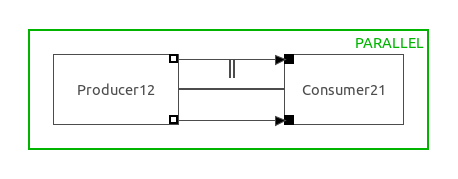
\includegraphics[scale=0.8]{./images/1_1-SystemDC_main.png}
  \caption{Composition of Producer and Consumer processes.}
 \end{subfigure}
 \begin{subfigure}{0.5\textwidth}
  \centering
	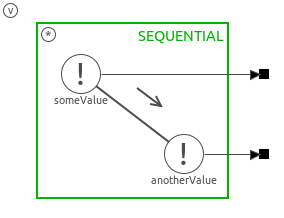
\includegraphics[scale=0.8]{./images/1_1-SystemDC_prod.png}
	\caption{The producer process.}
 \end{subfigure}%
 \begin{subfigure}{0.5\textwidth}
  \centering
	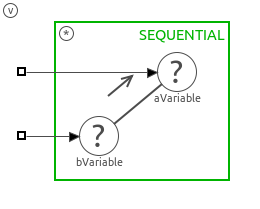
\includegraphics[scale=0.8]{./images/1_1-SystemDC_cons.png}
	\caption{The consumer process.}
 \end{subfigure}
  \caption{The producer-consumer (DC) model.}
  \label{fig:SystemDC}
\end{figure}

\begin{figure}
 \centering
 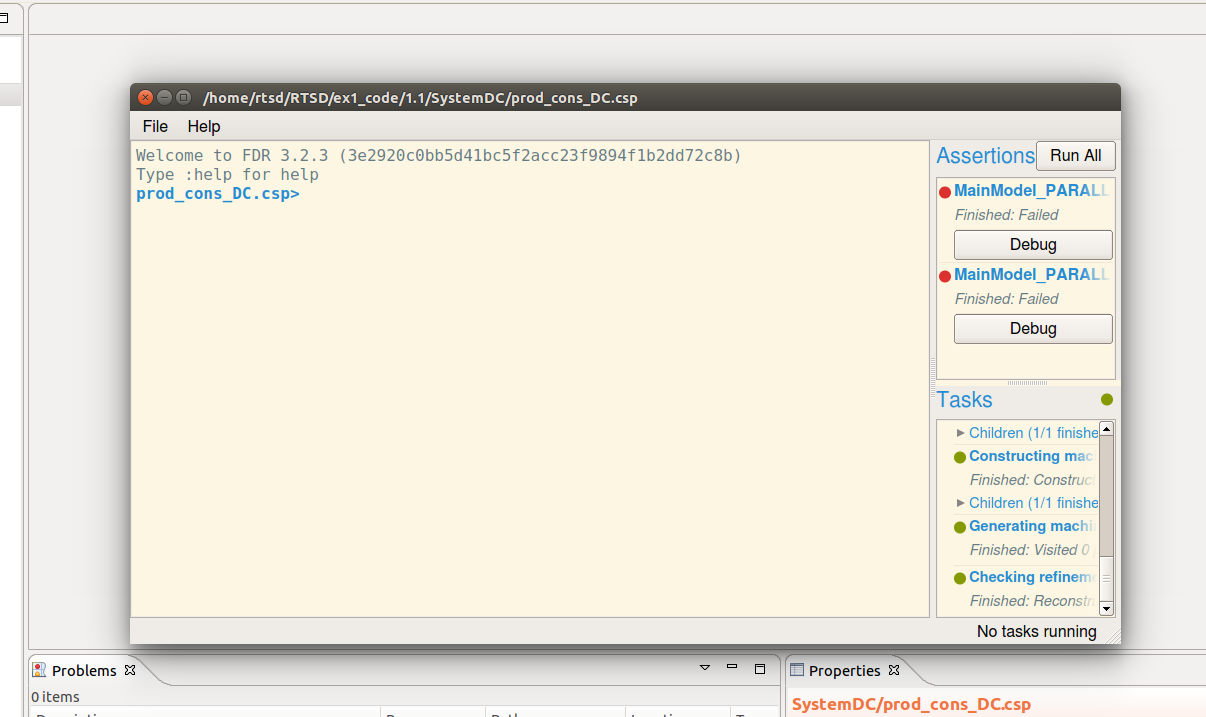
\includegraphics[width=\textwidth]{./images/1_1-SystemDC.png}
 \caption{Fails the tests in FDR.}
 \label{fig:FDR_DC}
\end{figure}

\FloatBarrier
\subsubsection{}
We extended the producer consumer (DF) model from figure~\ref{fig:SystemDF} with code blocks, and added \cpp implementation. The extended model is shown in figure~\ref{fig:SystemDF+} and the code in included in blocks \ref{code:1_2consumer} and \ref{code:1_2producer}. The initial few lines of the output is shown in figure~\ref{fig:SystemDF+_output}.

\begin{figure}
 \centering
  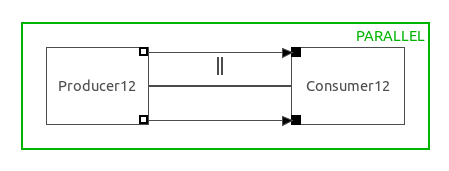
\includegraphics[scale=0.8]{./images/1_2-SystemDF+_main.png}
  \caption{Overview diagram of the producer consumer system.}
 \begin{subfigure}{0.5\textwidth}
  \centering
	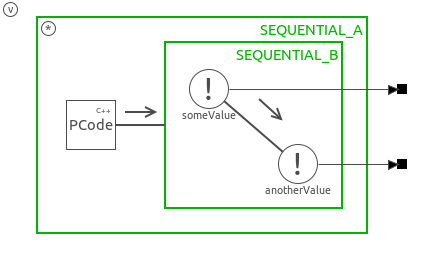
\includegraphics[width=\textwidth]{./images/1_2-SystemDF+_prod.png}
	\caption{The producer process.}
 \end{subfigure}%
 \begin{subfigure}{0.5\textwidth}
  \centering
	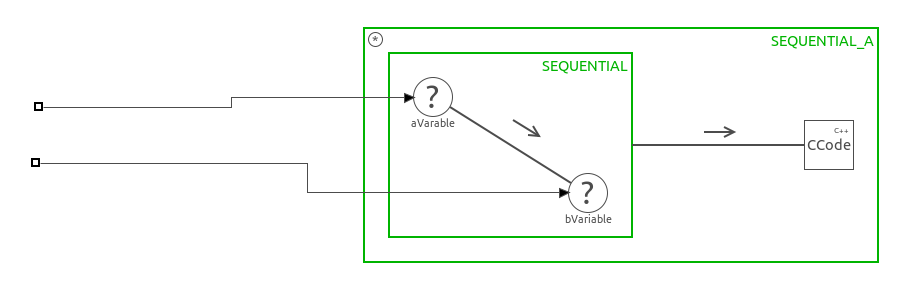
\includegraphics[width=\textwidth]{./images/1_2-SystemDF+_cons.png}
	\caption{The consumer process.}
 \end{subfigure}
 \caption{The producer-consuder (DF) model extended with code.}
 \label{fig:SystemDF+}
\end{figure}

\begin{lstlisting}[caption=Consumer12/CCode.cpp, label=code:1_2consumer, language=C++]
/**
 * Source file for the CCode model
 * Generated by the TERRA CSPm2LUNA generator version 1.1.1
 *
 * protected region document description on begin
 *
 * protected region document description end
 */

#include "Consumer12/CCode.h"
// protected region additional headers on begin
// Each additional header should get a corresponding dependency in the Makefile
// protected region additional headers end

namespace MainModel { namespace Consumer12 { namespace CCode { 

CCode::CCode(int &CCode_aVariable, int &CCode_bVariable) :
    CodeBlock(), CCode_aVariable(CCode_aVariable), CCode_bVariable(CCode_bVariable){
  SETNAME(this, "CCode");

  // protected region constructor on begin
  // protected region constructor end
}

CCode::~CCode()
{
  // protected region destructor on begin
  // protected region destructor end
}

void CCode::execute()
{
  // protected region execute code on begin
	if (this->CCode_aVariable == -1 || this->CCode_bVariable == -1)
		exit();
	else {
		printf("Receiving: CCode_aVariable: \t'%c'\n", this->CCode_aVariable);
		printf("Receiving: CCode_bVariable: \t'%c'\n", this->CCode_bVariable);

		printf("\n");
	}
  // protected region execute code end
}

// protected region additional functions on begin
// protected region additional functions end

// Close namespace(s)
} } } 
\end{lstlisting}


\begin{lstlisting}[caption=Producer12/PCode.cpp, label=code:1_2producer, language=C++]
/**
 * Source file for the PCode model
 * Generated by the TERRA CSPm2LUNA generator version 1.1.1
 *
 * protected region document description on begin
 *
 * protected region document description end
 */

#include "Producer12/PCode.h"
#include "string.h"
// protected region additional headers on begin
// Each additional header should get a corresponding dependency in the Makefile
// protected region additional headers end

namespace MainModel { namespace Producer12 { namespace PCode { 

PCode::PCode(int &PCode_anotherValue, int &PCode_someValue) :
    CodeBlock(), PCode_anotherValue(PCode_anotherValue), PCode_someValue(PCode_someValue){
  SETNAME(this, "PCode");

  // protected region constructor on begin
  // protected region constructor end
}

PCode::~PCode()
{
  // protected region destructor on begin
  // protected region destructor end
}

void PCode::execute()
{
  // protected region execute code on begin

	static int index = 0;

	char *stuff = "Appelflap";

	if (index == strlen(stuff)) {
		this->PCode_someValue = -1;
		this->PCode_anotherValue = -1;
	} else {
		this->PCode_someValue = stuff[index];
		this->PCode_anotherValue = stuff[index++];

		printf("Sending: PCode_someValue: \t'%c'\n", this->PCode_someValue);
		printf("Sending: PCode_anotherValue: \t'%c'\n", this->PCode_anotherValue);
	}


  // protected region execute code end
}

// protected region additional functions on begin
// protected region additional functions end

// Close namespace(s)
} } } 
\end{lstlisting}

\begin{figure}
 \centering
 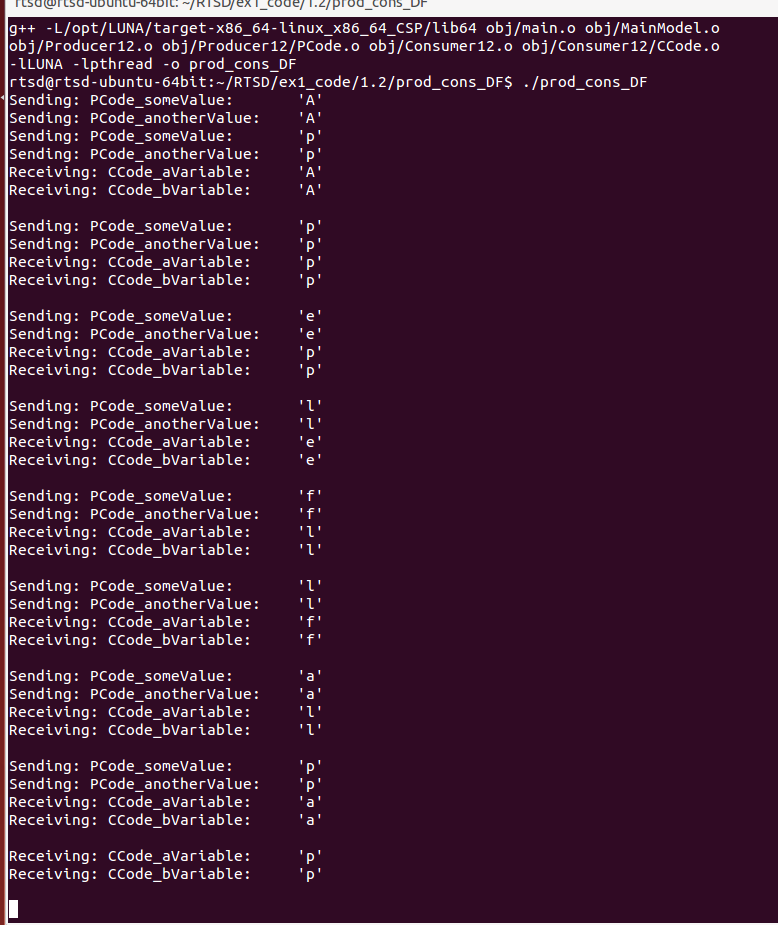
\includegraphics[width=\textwidth]{./images/1_2-SystemDF+_output.png}
 \caption{The output that our system produces.}
 \label{fig:SystemDF+_output}
\end{figure}
\FloatBarrier
\subsubsection{}
The consumer process cannot start before something is written on the channels. The producer process can start with the execution of its \cpp code. The parallel composition of the two processes can therefor only start with the execution of the \cpp code of the producer, hence the first two lines of the output originate from the producer.

Now, for the first channel, both the reader and the writer are available, and no other actions can be done by either process. The data is sent over the channel. After that, the same goes for the second channel.

Next, the producer can start over, starting with the execution of the \cpp code, but now the consumer can also execute its \cpp code. We expect either two lines of output produced by the producer's \cpp code, or two lines produced by the consumers \cpp code. And indeed we see the output of the producer's \cpp code.

Next, the writers in the producer cannot write to the channels, because the readers of the consumer are not ready. First the consumer's \cpp code needs to be executed before the process can recur and execute its readers. Hence the next two lines are produced by the consumer.

Now, the readers and writers do their thing and, again, either the producer's \cpp code can be executed, or the consumer's. We see for the complete initial part of the run that the producer's \cpp code is executed before the consumer's \cpp code.

\subsubsection{}
ProBE is an interpreter for CSPm scripts, the user can manually inspect the different execution paths that are possible. When a process is deadlock free, its execution paths are infinite. ProBE will never see the end of these executionpaths, nor will it know whether it has an end. FDR recognises this infinite behaviour, or more precise, it recognises finite behaviour. When it finds the process is able to terminate, it can show that the process fails the deadlock free-test. Similarly it can check for other properties without needing to simulate the complete execution paths likes ProBE does. ProBE can be used to inspect how a process deadlocks.

\subsubsection{}
If we addapt the \cpp code of the producer to start at the beginning of the word again when all characters have been sent, we can observe the behaviour of the process when it runs longer. We saw previously that the consumer only executed when the producer had to wait. This does not seem fair parallel. But when we watch what happens when the code runs longer, we occasionally see the consumer receive four values in a row, meaning that its \cpp code executed before the producer's \cpp code could prepare its next two values for the writers. So when both processes can execute, the parallel composition does not consistently execute one the them before the other. This seems fair.

\color{red}
Give proof that it is fair using the tools
\color{black}

\subsubsection{}
The composition $A ||| B$ does not deadlock. Whichever process gets to execute its \cpp code first, it will need to wait for the other process directly after. When both have executed their \cpp code, execution can continue by writing and reading on the channels.

\end{document}
